% Unofficial UChicago CS Poster Template
% v1.1.0 released September 8, 2022
% https://github.com/k4rtik/uchicago-poster
% a fork of https://github.com/anishathalye/gemini

\documentclass[final]{beamer}

% ====================
% Packages
% ====================

\usepackage[T1]{fontenc}
\usepackage{lmodern}
\usepackage[size=custom,width=120,height=72,scale=1.0]{beamerposter}
\usetheme{gemini}
\usecolortheme{uchicago}
\usepackage{graphicx}
\usepackage{booktabs}
\usepackage{bm}
%\usepackage{enumitem}
\usepackage{doi}
\usepackage[numbers]{natbib}
\usepackage[patch=none]{microtype}
\usepackage{tikz}
\usepackage{pgfplots}
\pgfplotsset{compat=1.18}
\usepackage{anyfontsize}
\usepackage{subcaption}
\usepackage{outlines}
\usetikzlibrary{arrows,shapes}

\pdfstringdefDisableCommands{%
\def\translate#1{#1}%
}

% ====================
% Lengths
% ====================

% If you have N columns, choose \sepwidth and \colwidth such that
% (N+1)*\sepwidth + N*\colwidth = \paperwidth
\newlength{\sepwidth}
\newlength{\colwidth}
\setlength{\sepwidth}{0.025\paperwidth}
\setlength{\colwidth}{0.3\paperwidth}

\newcommand{\separatorcolumn}{\begin{column}{\sepwidth}\end{column}}

% ====================
% Title
% ====================

\title{Modeling State of Health for a Li-On Battery}

\author{Karthik Nataraj (kartnat@stanford.edu) \and Hampus Carlens (hcarlens@stanford.edu) \and Julian Cooper (jelc@stanford.edu)}


% ====================
% Footer (optional)
% ====================

%\footercontent{
%  \href{https://www.example.com}{https://www.example.com} \hfill
%  CS229 Poster session, Stanford University --- XYZ-1234 \hfill
%  \href{mailto:alyssa.p.hacker@example.com}{alyssa.p.hacker@example.com}}
% (can be left out to remove footer)

% ====================
% Logo (optional)
% ====================

% use this to include logos on the left and/or right side of the header:
% \logoright{\includegraphics[height=7cm]{logo1.pdf}}


% ====================
% Body
% ====================

\begin{document}
\addtobeamertemplate{headline}{}
{
    \begin{tikzpicture}[remember picture,overlay]
     % \node [anchor=north west, inner sep=3cm] at ([xshift=0.0cm,yshift=1.0cm]current page.north west)
      %{\includegraphics[height=5.0cm]{logos/uc-logo-white.eps}}; % also try shield-white.eps
      \node [anchor=north east, inner sep=2.3cm] at ([xshift=0.0cm,yshift=2.5cm]current page.north east)
      {
\includegraphics[height=7.5cm]{stanford.png}};
    \end{tikzpicture}
}


\begin{frame}[t]
\vfill
\begin{block}{\large Motivation \& our dataset}
  % \centering
Lithium ion batteries are of great and increasing importance in today’s society due to their high energy density. Li-on batteries’ performance capability can be characterized by their State of Health (SOH). SOH is a measure of usable capacity over rated capacity. Accurately predicting how many cycles a battery can perform before reaching 80\% of rated capacity (Remaining Useful Life (RUL)) is important for reliability. While much work has already been done in this space to accurately predict RUL, recent studies (\cite{energiesMdpi}, \cite{DariusOld})  have called for further research into white box models that predict the SOH curve to enable deployment for online systems.    
In this project, we develop a scalable (and explainable) \textbf{white box model to predict the SOH curve until 80\% threshold} (as opposed to a point estimate of RUL) given the first 100 cycles. Since our predicted SOH curve implies an RUL prediction, we also compare our implied RUL prediction error to that of previous studies.
\newline

The \href{https://data.matr.io/1/projects/5c48dd2bc625d700019f3204}{\textbf{dataset}} \textbf{we have selected contains approximately 96,700 cycles (approx. 780 cycles per battery for 124 batteries)}. For each cycle the authors captured voltage, applied current and temperature sampled at 2.5 second intervals. This is the largest publicly available dataset for identical commercial lithium-ion batteries cycled under controlled conditions, and is the same source used by two recent papers that motivated our project: “Machine learning pipeline for battery state-of-health estimation” (Nature, 2021)\cite{roman2021machine} and "Data-driven prediction of battery cycle life before capacity degradation" (Nature, 2019)\cite{severson2019data}.
\end{block}

% \begin{frame}[t]
\begin{columns}[t]
\separatorcolumn

\begin{column}{\colwidth}

  \begin{block}{1. Neural Network}
            
Our Neural Network model predicts RUL of a battery given data features derived only from its first 100 cycles. The purpose was
to improve results from \cite{severson2019data} and perform feature importance analyses to inform subsequent time series and Bayesian Inference
models.

\begin{enumerate}[(a)]%[label=(\alph*)]
 \item \textbf{Architecture}: 2-layer feed-forward, densely connected neural network.  First layer had 1076 neurons and the second 96. We then used the learning rate of .001 with the Adam optimizer, ReLU activation, and full-batch gradient descent (since the training dataset is already small).  Training and validation: 81 batteries; Test: 43
 \item \textbf{Feature engineering}: Due to slow training convergence and poor performance despite l1/l2 regularization, condensed original derived feature set of \cite{severson2019data} consisting of 20 features, to a total of 3, using Shapley values ((a) of Figure \ref{fig:birds}): variance of difference in charge curves, average temperature and current
\end{enumerate}

    \begin{minipage}[t]{0.65\textwidth}
    \textbf{Results}. Obtained training RUL MAPE $\approx 8.6 \%$, test RUL MAPE $\approx 10.8 \%$, better than the best model of \cite{severson2019data}, which obtained test MAPE $13 \%$.
    \end{minipage}
    \begin{minipage}[t]{0.30\textwidth}
    \begin{flushright}
    \begin{tabular}{ l c }
       \textbf{MAPE RUL} &  \textbf{10.8\%}
    \end{tabular}
    \end{flushright}
    \end{minipage}
    
    \begin{figure}[H]
% \captionsetup{font=footnotesize}
     \centering
     \begin{subfigure}[b]{0.5\textwidth}
         \centering
         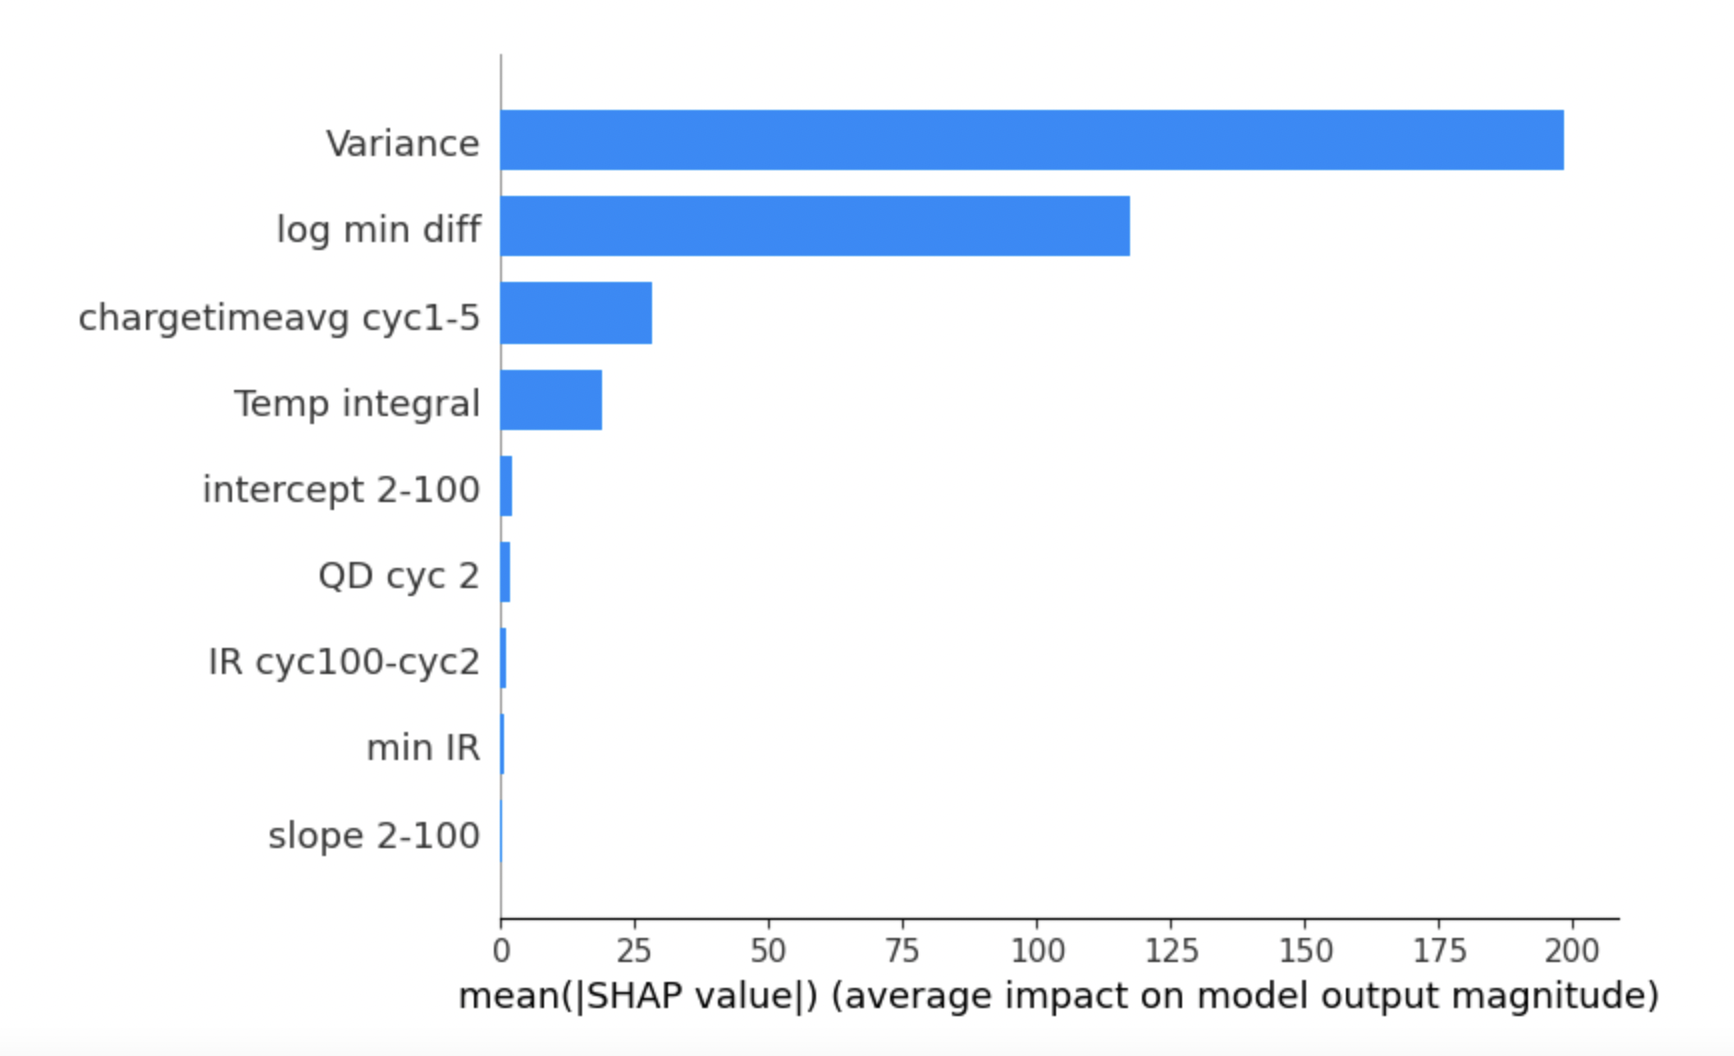
\includegraphics[width=\colwidth/2,height = 12cm]{figs/shap.png}
         \caption{Feature importance for non time-series variables}
         %\label{fig:y equals x}
     \end{subfigure}
     \hfill
     \begin{subfigure}[b]{0.49\textwidth}
        \centering
        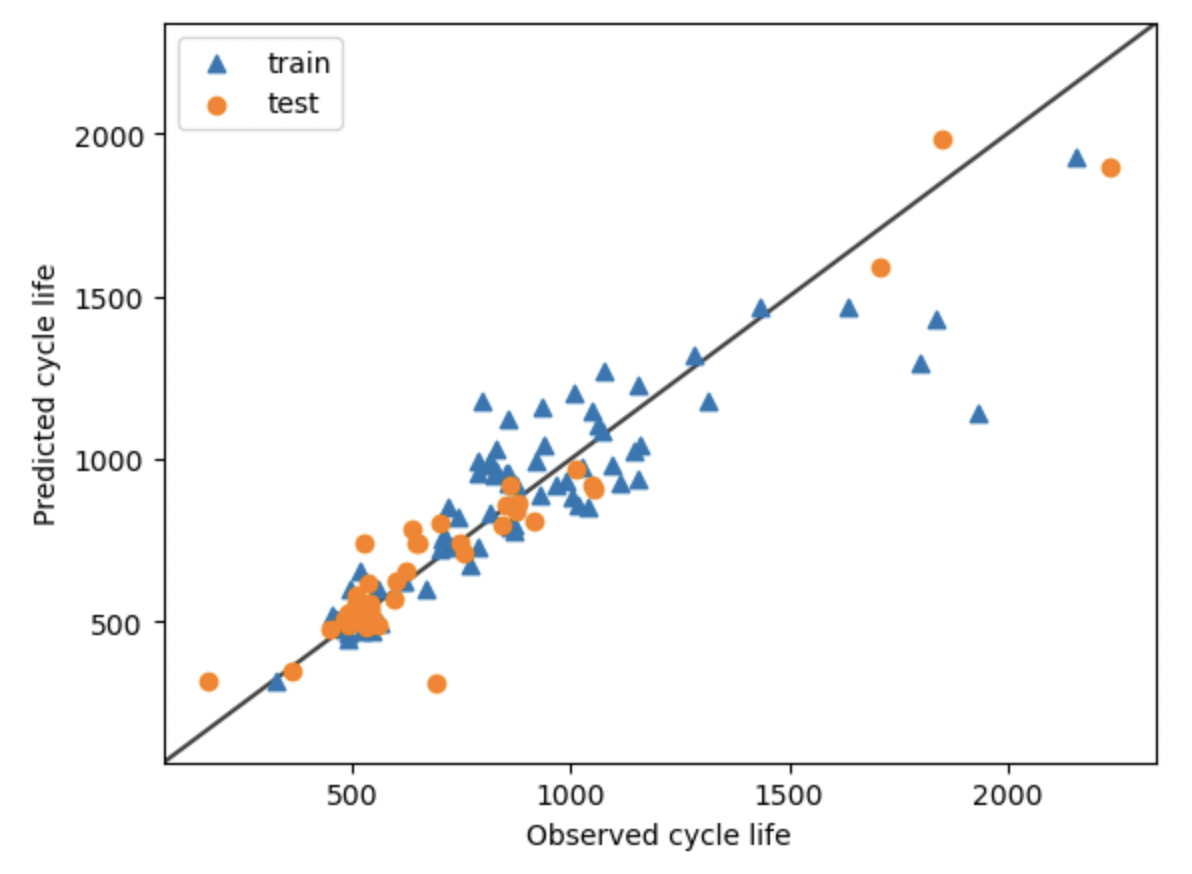
\includegraphics[width=\colwidth/2,height = 12cm]{figs/obspred.png}
         %\caption{\textbf{Predicted vs. Actual cycle lives}}
         %\label{fig:three sin x}
        %\caption{}
        %\label{fig:birds1}
         %\centering
         %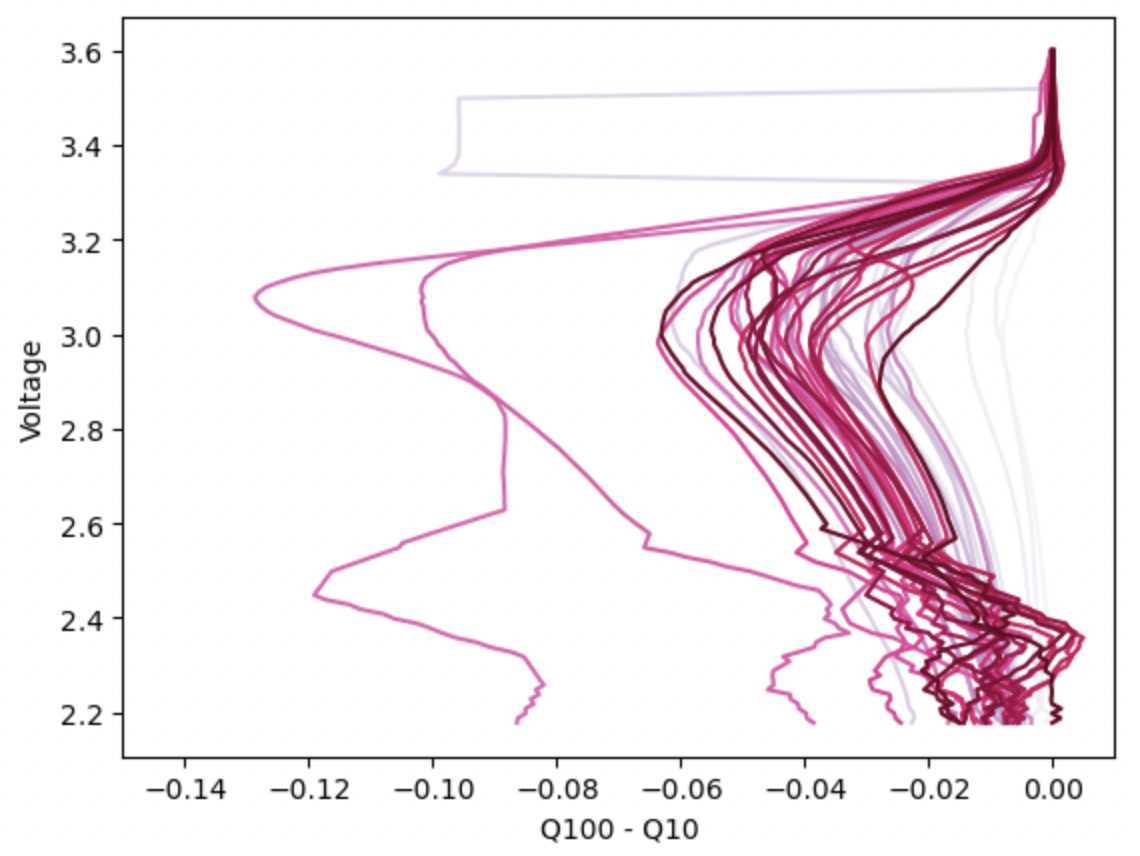
\includegraphics[width=\textwidth,height = 5cm]{figs/variance.png}
         \caption{Predicted vs. actual cycle life for test set batteries}
         %\label{fig:three sin x}
     \end{subfigure}
\caption{Descriptive plots for neural network approach to predicting} %cycle life}
\label{fig:birds}
\end{figure} 

  \end{block}

\begin{alertblock}{\small Discussion and takeaways}

\begin{itemize}

 \item Even with an small training dataset it was possible to improve performance of a regularized linear model with shallow neural networks, using a very small sample of very good features.
 \item Eliminating noisy features proved more helpful in improving performance than hyperparameter tuning. Our dataset was too small to support significant hyperparameter calibration, even with cross-validation techniques. 
 \item \textbf{Next steps}: Going forward we'd focus on decay curve predictions using LSTM networks, given the partial success of ARIMA models (see next column)

\end{itemize}

\end{alertblock}

\end{column}

\separatorcolumn

\begin{column}{\colwidth}

  \begin{block}{2. Auto-regression (ARIMA)}

    The purpose of using time series models was to predict the entire capacity degradation curve, not only the RUL as with the neural net. The ARIMA model considered only one measurement per cycle, the discharge capacity $Q_D$ and from a machine learning point of view there was a separate model for each battery. 
    
    \begin{enumerate}[(a)]%[label=(\alph*)]
      \item \textbf{Choice of hyperparameters} was done through Box-Jenkins method which is based on autocorrelation and partial autocorrelation. The results were then sense checked using an automatic parameter selection algorithm called auto-ARIMA. We found that p=2, d=2, q=2 worked well, and in particular that our results were very sensitive to d being at least 2.
      
      \item \textbf{Exogenous variables}; ARIMA models can be used with or without exogenous variables. We tried adding exogenous variables to the ARIMA model, however, since the battery life cycles were of different lengths it was hard to consistently apply exogenous variables in training and testing. We ended up not using exogenous variables. 
    \end{enumerate}

    \begin{minipage}[t]{0.65\textwidth}
    \textbf{Results} Fit evaluation using ARIMA(2,2,2) on out-of-sample test batteries given information from the first 100 cycles only.    
    \end{minipage}
    \begin{minipage}[t]{0.30\textwidth}
    \begin{flushright}
    \begin{tabular}{ l c }
       \textbf{MSE SOH} &  \textbf{0.049} \\
      % \hline
       \textbf{MAPE RUL} &  \textbf{26.5\%}
    \end{tabular}
    \end{flushright}
    \end{minipage}
      
    \begin{figure}[H]
     \centering
     \begin{subfigure}[b]{0.5\textwidth}
         \centering
         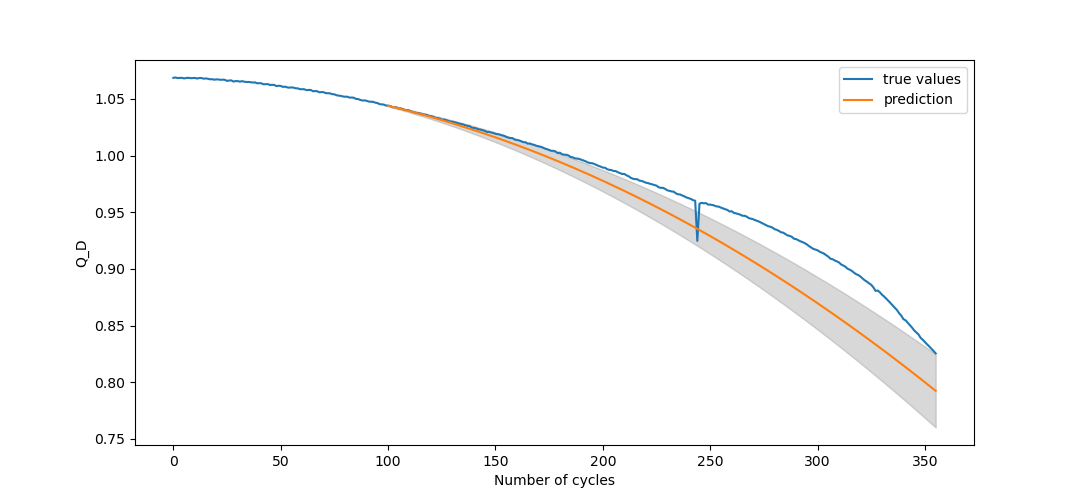
\includegraphics[width=\colwidth/2,height = 12cm]{figs/best fit 100.png}
         \caption{Good prediction example on test battery}
         %\label{fig:y equals x}
     \end{subfigure}
     \hfill
     \begin{subfigure}[b]{0.49\textwidth}
        \centering
        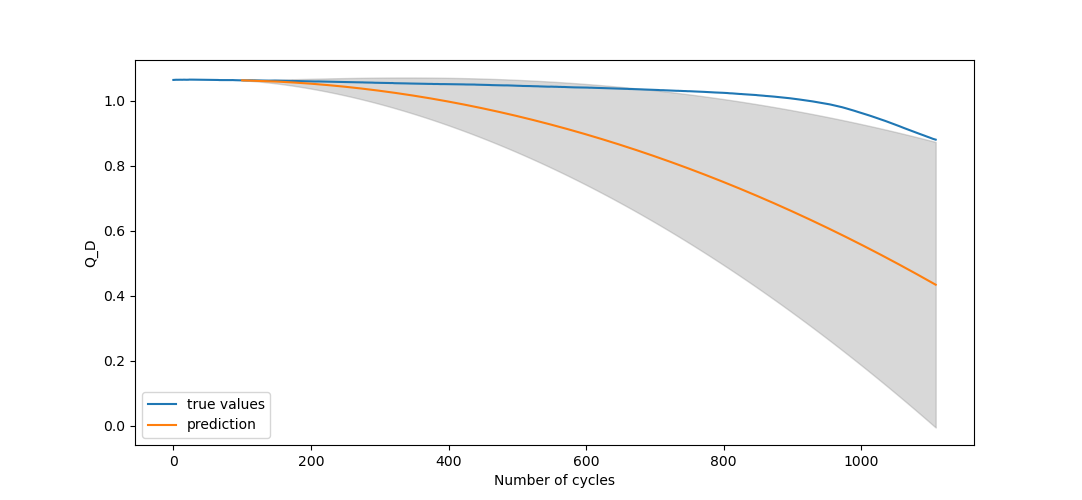
\includegraphics[width=\colwidth/2,height = 12cm]{figs/worst fit 100.png}
         \caption{Poor prediction example on test battery}
         %\label{fig:three sin x}
     \end{subfigure}
\caption{Predicted discharge capacity over cycle life until 0.8 threshold} %cycle life}
\label{fig:birds}
\end{figure} 

  \end{block}

  \begin{alertblock}{\small Discussion and takeaways}
  \begin{outline}
      \1 The ARIMA model results had a very large variance, as seen in Figure (2).
      \1  It was almost impossible to estimate any 1000+ cycle battery life using just 100 cycles. However, battery cycle lives of 300-700 were possible to estimate with reasonable accuracy.
      \1 The largest limitation of the model was the inability to learn across batteries.  
      \1 \textbf{Next steps}: Future work could focus on implementing exogenous variable to impose data priors on the algorithm. This could include an RUL estimation from the neural network combined with a generic decay curve.
  \end{outline}
     

  \end{alertblock}
\end{column}

\separatorcolumn

\begin{column}{\colwidth}

\begin{block}{3. Bayesian inference model}
    We explored Bayesian Inference as a way to impose more known physics on the problem. Main idea: since we know the discharge capacity curve of each battery must be a decay curve, why don't we specify such a functional form and only ask our model to learn the shape and translation. 

    \begin{enumerate}[(a)]%[label=(\alph*)]
        \item \textbf{Functional form}: We selected an inverse sigmoid $\hat{y} = \gamma - 1 / 1+\exp(-\alpha(x-\beta))$ because it described our data well in the region of interest (y = 0.8 to 1.2) and its parameters (shape, translation, y-asymptote) were highly interpretable. 
        
        \item \textbf{Parameterization}: Relating parameters $\alpha, \beta, \gamma$ to features $x_i$ identified by Neural Network:
        % We choose linear models for $\alpha$ (= $a^\top x$) and $\beta$ (= $b^\top x$) based on the effectiveness of the linear model from \cite{severson2019data} for predicting RUL (closely related to translation in our case). Then for $\gamma$ we further restrict our formulation by specifying that the y-asymptote must equal the nominal discharge capacity ($x_1$).
        \begin{align*}
            \alpha & = a_0 + a_1 x_1 + a_2 x_2 + a_3 x_3 + a_4 x_4 + a_5 x_5 && \text{linear model for rate of decay}\\
            \beta & = b_0 + b_1 x_1 + b_2 x_2 + b_3 x_3 + b_4 x_5 + b_5 x_5 && \text{linear model for horizontal translation}\\
            \gamma & = x_1 && \text{asymptote set to nominal discharge capacity}
        \end{align*}
        
        \item \textbf{Prior specification}: We assume that our labels $y$ are generated from a gaussian with mean $\hat{y}$ (our predictions) and variance $\sigma^2 \sim \text{Gamma}(2,1)$. Informative intercept priors $a_0 \sim N(3,1)$, $b_0 \sim N(2,1)$ (empirically estimated) and standard normals for $a_i, b_i \sim N(0,1)$ $i = 1, 2, ..., d$.
        % $$ y &\sim \text{Normal}\left(\gamma - 1 / 1+\exp(-\alpha(x-\beta)), \sigma^2 \right), \quad \sigma^2 \sim \text{Gamma}\left(1, \quad 2 \right) $$
    \end{enumerate} 
    
    \begin{minipage}[t]{0.65\textwidth}
    \textbf{Results} Fit evaluation on out-of-sample test batteries given information from the first 100 cycles only. 
    \end{minipage}
    \begin{minipage}[t]{0.30\textwidth}
    \begin{flushright}
    \begin{tabular}{ l c }
       \textbf{MSE SOH} &  \textbf{0.015} \\
      % \hline
       \textbf{MAPE RUL} &  \textbf{33.5\%}
    \end{tabular}
    \end{flushright}
    \end{minipage}
    
    \begin{figure}[H]
        \centering
        \begin{subfigure}[b]{0.49\linewidth}
            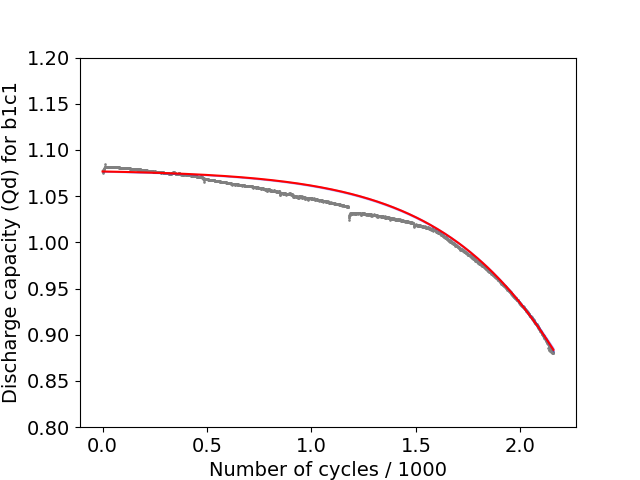
\includegraphics[height=12cm,width=\linewidth]{figs/bayes_plot_with_error_b1c1.png}
            % \caption{SOH MSE = 0.0008, RUL MAPE = 1.5\%}
            \caption{Good prediction example on test battery}
            \label{fig:bayessub1}
        \end{subfigure}
        \begin{subfigure}[b]{0.49\linewidth}
            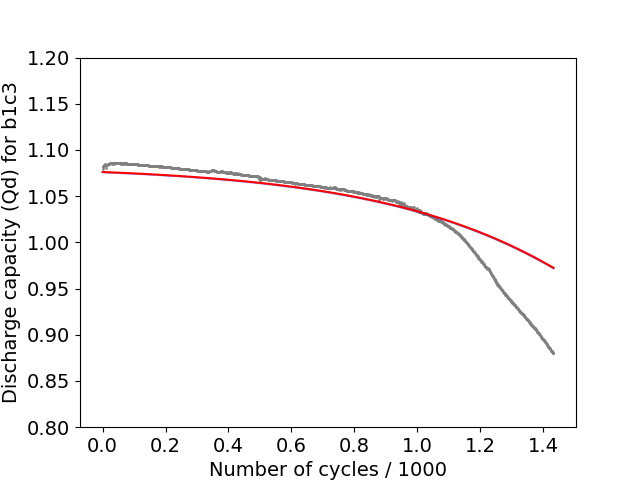
\includegraphics[height=12cm,width=\linewidth]{figs/bayes_plot_with_error_train_b1c3.png}
            % \caption{SOH MSE = 0.022, RUL MAPE = 38.5\%}
            \caption{Poor prediction example on test battery}
            \label{fig:bayessub2}
        \end{subfigure}
        \caption{Predicted discharge capacity over normalized cycle life}
        \label{fig:bayespred}
    \end{figure}
\end{block}
    \begin{alertblock}{\small Discussion and takeaways}

    \begin{itemize}
    \item Our model predicts well for batteries with mid-long cycle lives (Figure \ref{fig:bayessub1}), but often overshoots for short cycle life batteries (e.g. Figure \ref{fig:bayessub2}).
    
    \item This is partly due us having so few short cycle life training observations (variance), but also may be indicative of inflexibility in the model parameterization (bias).
    
    \item \textbf{Next steps}: We use a linear model to parameterize $\alpha$ and $\beta$, but a deeper understanding of the physics involved might lead us to specify something different (e.g. interaction terms).
    
    \end{itemize}


  \end{alertblock}

\end{column}

\separatorcolumn
\end{columns}
\vfill
\begin{block}

    \nocite{*}
    \footnotesize{\bibliographystyle{plainnat}\bibliography{poster}}

\end{block}

\end{frame}

\end{document}